% Chapter Template

\chapter{SparkSQL Server in Practice: Scan Sharing} % Main chapter title

\label{Chapter4} % Change X to a consecutive number; for referencing this chapter elsewhere, use \ref{ChapterX}

\lhead{Chapter 4. \emph{SparkSQL Server in Practice: Scan Sharing}} % Change X to a consecutive number; this is for the header on each page - perhaps a shortened title

%----------------------------------------------------------------------------------------
%	SECTION 1
%----------------------------------------------------------------------------------------

\section{Scan Sharing}

In large data warehouses, companies, users submit their queries at the same period of time. There are some files which are "hotter" since they are used more frequently than the others, then reading those files multiple times from disk can be redundant by reading each file only one time and many others users can use them. Sharing scan does not only help to reduce the reading cost but also the communication cost, then the total execution time of the queries is reduced.\\

We instantiate the sharing scan technique into our system by using two approaches, one from MRShare \cite{nikiel2010} works and the other is a feature of Spark itself. Both techniques are easily to implement and integrate into our system, which proves the generalization and extensibility of our system.

%-----------------------------------
%	SUBSECTION 1
%-----------------------------------
\subsection{Current State-of-the-Art}

As described before,  on Apache Spark, there is no published work on Work Sharing. The current State-of-the-art of Scan Sharing on Apache Hadoop MapReduce is MRShare.\\
MRShare is a sharing framework, which provides two techniques of sharing: map input sharing and map output sharing. The idea of MRShare is group the jobs which can share map input or map output into groups, with the constrains of maximizing the total saving by defining their own cost model.\\

Grouping jobs into one is not always beneficial since the reading cost is decreased but the amount of data shuffled over networks may increased. Using dynamic programming and a cost model, MRShare evalutates possible groups and decides which groups give it the maximum saving.\\
The technique that MRShare uses to merge multiple jobs into one called simultaneous pipeline. It attaches a tagging in each tuple to identify which job it belongs to.\\
%-----------------------------------
%	SUBSECTION 2
%-----------------------------------

\subsection{Caching in Apache Spark}

%----------------------------------------------------------------------------------------
%	SECTION 2
%----------------------------------------------------------------------------------------

There is an important feature on Apache Spark which is Caching. This feature utilizes the memory storage to keep data in memory and uses it multiple times. When multiple jobs in a Spark Application use the same input file, we can cache the partitions which are hold the input file at the first job. When the second job wants to do some transformations on those partitions, it does not need to recompute from scratch to get them, it just checks if they are in memory or not, if they are in memory, it gets them and applies transformations on them.\\

Caching is a costly operation itself. If the cost of caching is larger than the cost of reading input files multiple times, so caching is not beneficial. In addition, if memory storage of the cluster is not large enough to cache the whole input files, it may write a part of the input files to disk and read them when needed, which also increases the I/O cost.\\
		
\section{Scan Sharing in SparkSQL Server}
We integrate two techniques of scan sharing: using MRShare and using caching. \\
\textbf{At client side}, since MRShare requires some pre-defined parameters about the jobs, when users submit their Spark applications through the spark-submit command, they need to pass those parameters too.\\

\textbf{At server side}, we only discuss about the components that we need to plug our own implementations for scan sharing:
\begin{itemize}
\item WorkSharing Detector: we need to add our own Rule which is "ScanSharing" to detect which jobs can be shared scan.
\item CostModel: for MRShare, we implement the cost model that was published in the paper. For caching technique, currently, there is no pulished works about cost model relates to caching data in memory, it is going to be a part of our future work, currently, we do not add the cost model for caching.
\item Optimizer: for MRShare, the dynamic programming algorithms which are described in the original paper are implemented with some modifications to adapt and can be integrated into our system. Since we do not have the cost model for caching technique, currently, we just output the same batch of jobs as the same as the input batch of jobs.
\item Rewriter: We add two Rewrite rules. For MRShare, we add the simultaneous rewrite rule. For caching, we add the caching rewrite rule. The details of the implementations of simultaneous pipeline technique is described in the next section. The rewrite rule for caching is simple since we cache scan RDD of the first job in the batch, then replace the scan RDD of the rest jobs in the batch with the cached scan RDD.
\item PostScheduler: At the moment, we use FIFO strategy for MRShare technique, while in caching technique, it should be noticed that the first job which does the caching of scan RDD needs to be executed first, then we apply FIFO strategy for the rest jobs in the batch.
\end{itemize} 

\section{Implementations}

Caching is a feature of Apache Spark which is widely used. Besides that, the cost model and dynamic programming algorithms are well described in the MRShare paper. In this section, we mainly discuss about how we implement the simultaneous pipeline technique used in MRShare. In addition, we also briefly describe the MRShare dynamic programming and how we implement it.

\subsection{MRShare Cost Model and Its Algorithms}
The general idea of MRShare for scan sharing is to merge a batch of MapReduce jobs into one job which is called metajob. MRShare Cost Model shows that greedily merging jobs is not always beneficial since it also adds the extra sorting costs and also the shuffle bytes over the network.\\
The optimization problem of MRShare is formulated as: \textit{Given a set of jobs J = {J1, ..., Jn}, groups the jobs into S non-overlapping groups G1, G2, ... , Gs, such that the overall sum of savings is maximized.} The authors prove that this is an NP-hard problem so they consider a relaxed version when the extra sorting overheads relies only on the job that contains the highest map output ratio in a group. They realize that if all the jobs in a group are sorted into a list according to the map output ratio, the optimal grouping will consist of consecutive jobs in the list. The problem is become as splitting the sorted list of jobs into sublists which give the maximized savings.\\
The authors propose an dynamic, exact programming algorithm called \textit{SplitJob}: suppose in the optimial arrangement, the last sublist starts from job Ji, we need to find out the optimal arrangement for the previous i-1 jobs. It will search all the possible cases for job Ji-1. The pseudo code is provided below.

\begin{algorithm}
\caption{SplitJob(J1, ... , Jn)}
%\begin{algorithmic}[1]
1. Compute GAIN(i,l) for  $1 \leq i \leq l \leq n$. \newline
2. Compute GS(i,l) for  $1 \leq i \leq l \leq n$. \newline
3. Compute c(l) and source(l) for $1 \leq l \leq n$. \newline
4. Return c and source.
%\end{algorithmic}[1]
\end{algorithm}

The map output ratio is measured from processed-jobs and kept in history so user can pass them through the modified version of spark-submit command that we provide. Since the output of \textit{SplitJob} can contain group of single jobs, so a refinement algorithm called \textit{MultiSplitJob} is proposed. The main idea of \textit{MultiSplitJob} is to put those single jobs from \textit{SpiltJob} into a new job list and apply again \textit{SplitJob} on it. The pseudo code is provided below.

\begin{algorithm}
\caption{MultiSplitJob(J1, ... , Jn)}
$J \leftarrow {J1, ... , Jn}$ (input jobs) \newline
$G \leftarrow \emptyset$ (output groups) \newline
\While {($J \neq \varnothing$)} {
	compute $\delta${j} for each $Jj  \in J$ \newline
	ALL = SplitJobs(J) \newline
	$G \leftarrow G \cup ALL.getNonSingletonGroups()$ \newline
	$SINGLES \leftarrow ALL.getSingletonGroups()$ \newline
	\eIf {($|SINGLES| < |J|$)} {
		$J \leftarrow SINGLES$
	} {
		Jx = SINGLES.theSmallest() \newline
		$G \leftarrow G \cup {Jx}$ \newline
		$J \leftarrow SINGLES \setminus Jx$ \newline
	}
}
return G as the final set of groups
\end{algorithm}

\subsection{Simultaneous Pipeline Technique}

In general, this technique is used when merging multiple jobs read the same input file into one meta job. The technique has been used in Multi Query Optimization of Apache Pig. In MRShare, they proposed this technique on Hadoop MapReduce as an automatic module. On Apache Spark, to the best of our knowledges, all the query optimizations are currently focusing on single query, not multi query. We reintroduce the simultaneous pipeline technique and implement it on Apache Spark.

There are 4 new RDDs that we create to implement the technique.
\begin{itemize}
\item MuxRDD: The MuxRDD is used to buffer the input record and multiplex it into multiple pipelines, which represent multiple jobs.
\item LabellingRDD: The LabellingRDD is used to attach the label into each tuple before it is shuffled over the network. The label is an integer which is attached to the key of the tuple. So, the old tuple [Key, Value] becomes [(Label, Key), Value].
\item DispatchRDD: The DispatchRDD is used to route the tuple to the right pipeline by using the label attached inside it.
\item PullRDD: Because Spark is based on Pull Mechanism, which means the child RDD asks its parent RDDs to give it the tuple. In default, the saveAsTextFile action has the puller to trigger the job. To keep Spark at it is, we create our new puller called PullRDD.
\end{itemize}

We also modify some parts of the shuffle component on Apache Spark:
\begin{itemize}
\item ShuffledRDD: the ShuffledRDD contains only one Aggregator, the object holds the aggregate function. In our case, to merge multiple jobs which have different Aggregators, we create a list of Aggregators to hold their Aggregators.
\item ExternalSorter: before writing to files and shuffling them over the network, Spark does a local aggregation (it is a combiner in Hadoop MapReduce), so we also need to apply the correct aggregate function to the tuple by checking the label attached into it.
\item AppendOnlyMap: when the aggregation happens in the other stage after getting the data over the network (in Hadoop MapReduce, it is the Reduce phase), again, we need to apply the correct aggregate function to the list of tuple by checking the label attached into it.
\end{itemize}

We provide two examples to demonstrate how simultaneous pipeline technique works. Two jobs are described at two figures below. For each figure, on the left are two original DAGs and on the right is the meta DAG which is merged from those two DAGs.

\begin{figure}
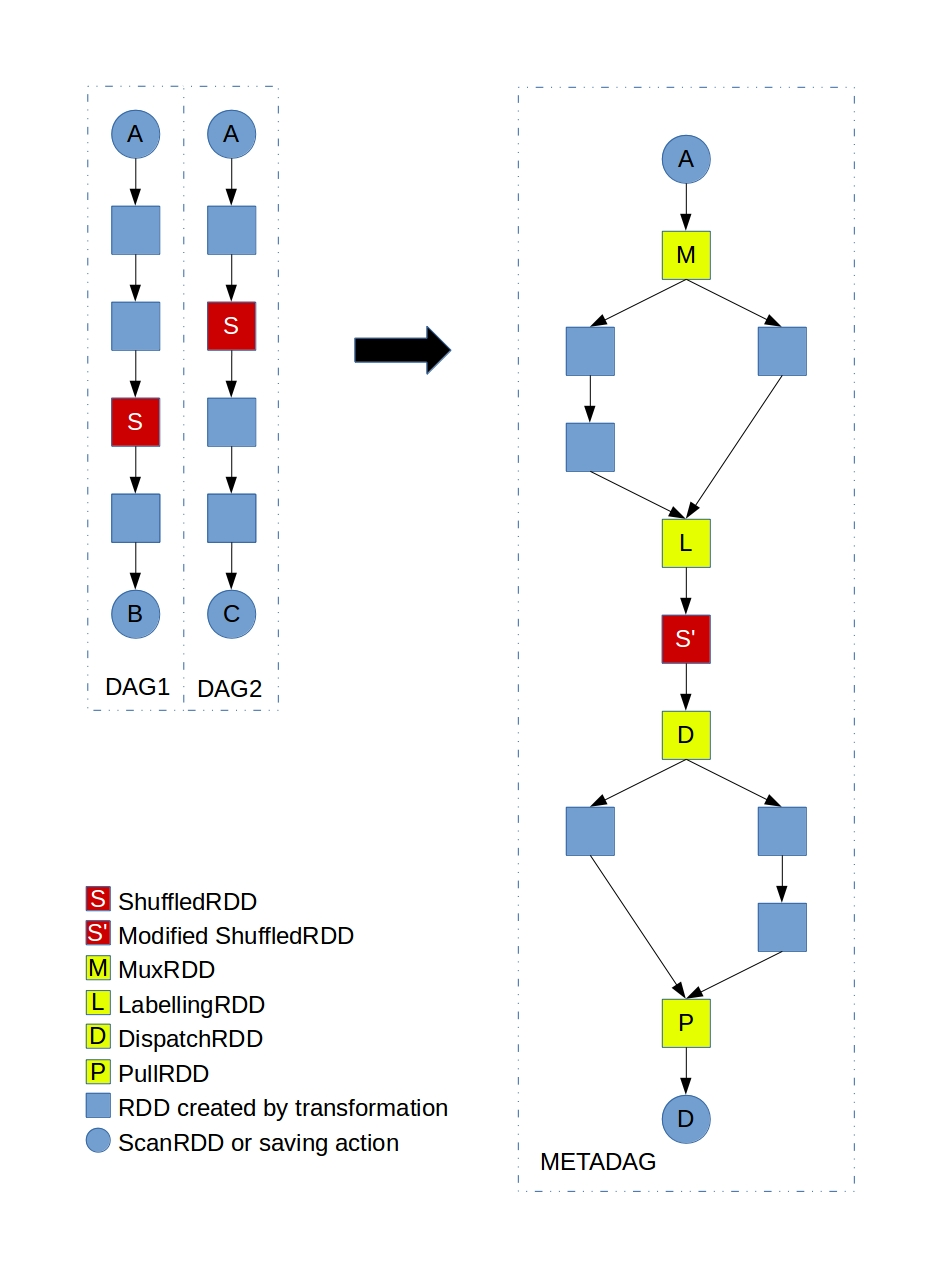
\includegraphics[width=\textwidth]{Figures/singlemetajob.jpg}
\caption{Transformation process of a simple case}
\label{fig:simplemetajob}
\end{figure}

\begin{figure}
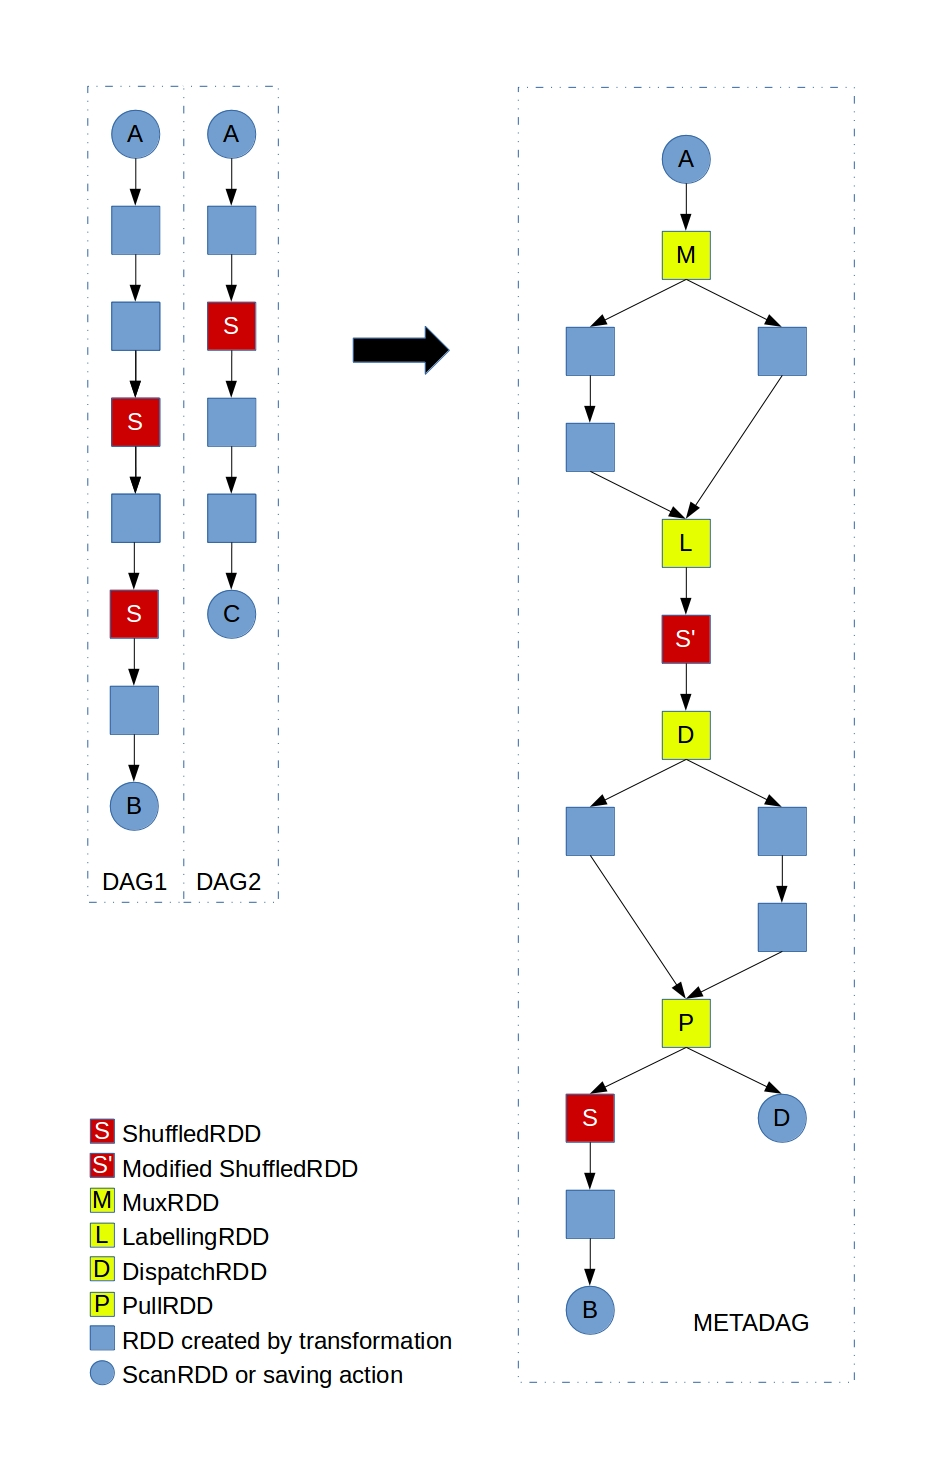
\includegraphics[width=\textwidth]{Figures/complexmetajob.jpg}
\caption{Transformation process of a complex case}
\label{fig:complexmetajob}
\end{figure}

\begin{itemize}
\item Two jobs, each job has only one ShuffleRDD
From figure \ref{fig:simplemetajob}, we can see the metajob is a DAG which is mainly composed from the two original DAGs. The MuxRDD is attached right after the scan RDD, it does the multiplexing the input into two pipelines. Before going to the ShuffleRDD, a LabellingRDD is inserted right before the ShuffleRDD to attach the label into each tuple. In this example, we have two jobs, so the label has two values which is 0 and 1. The ShuffledRDD is modified so it contains two aggregate functions. The aggregation before and after shuffling happens on the correct tuple with the correct aggregate function due to the label attached into each tuple. The DispatchRDD is attached after the ShuffledRDD and routes the correct tuple to the associated pipeline by the label attached into each tuple. The PullRDD is inserted at last to do the pull and trigger the whole job, then saves the output to disk storage.
\item Two jobs, one job has two ShuffleRDDs
The part of DAG1 from the beginning up to the second ShuffledRDD and DAG2 are merged as the same way as the case above. The difference is that the PullRDD just saves a part of data comes from the pipeline of DAG2, PullRDD is also followed by the rest part of DAG1 and saves to disk storage when finishes. The process is described in figure \ref{fig:complexmetajob}
\end{itemize}

This technique is embedded into Spark Source Code and is an automatic feature of SparkSQL Server. In those two examples, we just discuss about two simple cases that can happen when using MRShare and simultaneous pipeline technique, but the more complex DAGs can also be merged into one meta job automatically.\\

In order to implement the simultaneous pipeline technique, we need to have a deep understanding of Spark internal and its dataflow. A modified Spark is needed to make our system work properly, so if user want to use our system, they need to use our provided Spark. Details are descibed in \ref{AppendixA}